\chapter{APPROCHE MÉTHODIQUE ET MODÉLISATION}
\begin{spacing}{1.2}
\minitoc
\thispagestyle{MyStyle}
\end{spacing}
\newpage

L’évaluation de la réussite des étudiants est une préoccupation majeure dans le domaine de l’enseignement. L'utilisation de l'intelligence artificielle, en particulier l'apprentissage automatique, s'est révélée être un outil puissant pour aborder ce défi. De nombreuses études ont exploré l'application de techniques d'apprentissage automatique dans la prédiction des performances académiques des étudiants, cherchant à identifier les facteurs clés qui influencent le succès universitaire. \\
C'est dans cette perspective que ce chapitre consistera à aborder l'état de l'art sur la prédiction de réussite des étudiants, une approche de solution, et la modélisation de notre solution pour prédire la réussite en licence économie à l'UNZ en utilisant l'intelligence artificielle.

\section{État de l'art}
De nombreuses études ont été menées pour prédire avec précision la réussite des étudiants, afin de mettre en place des mesures d'intervention précoce et d'améliorer les politiques éducatives. L'utilisation de l’intelligence artificielle dans ce domaine a produit des résultats prometteurs. Cette section passe en revue les principales études antérieures sur la prédiction des réussites des étudiants, mettant en évidence les méthodes et techniques utilisées, ainsi que les défis et limitations rencontrés.

\subsection{Études antérieures sur la prédiction des réussites des étudiants}
La prédiction de la réussite des étudiants a été abordée par de nombreuses études à travers le monde. Ces études ont généralement utilisé une variété de techniques, allant des modèles statistiques traditionnels aux approches plus récentes basées sur l'apprentissage automatique et l'intelligence artificielle. Parmi les études les plus remarquables, celles-ci se sont concentrées sur l'utilisation de données démographiques des étudiants, telles que le sexe, l'âge et le niveau socio-économique, ainsi que sur les performances académiques antérieures, telles que les notes et les résultats aux examens standardisés.

Dans une étude menée par \textbf{Jean-Philippe Vandamme}, \textbf{Nadine Meskens} et \textbf{Abdelhakim Artiba}, l'échec scolaire en première année universitaire a été le sujet central de recherche \cite{vandamme2023comparison}. Cette problématique a suscité de nombreux débats parmi les psychopédagogues qui ont cherché à la comprendre et à l'expliquer, tandis que les statisticiens se sont attelés à le prévoir.
L'objectif de leurs recherches était de développer un modèle permettant de déterminer, dès le début de l'année universitaire, le groupe d'étudiants de première année qui nécessitait prioritairement des ressources pédagogiques pour améliorer leur taux de réussite. Pour ce faire, ils ont élaboré un questionnaire basé sur les hypothèses posées dans de nombreux modèles théoriques, puis ils ont collecté des données diverses et nombreuses à l'aide de ce questionnaire.
Ensuite, à l'aide de méthodes statistiques ou de fouille de données (data mining\textsuperscript{} \footnote{\textbf{Data mining} est l'analyse de données volumineuses pour trouver des corrélations, des patterns et du savoir.}), leur objectif était d'extraire des informations permettant de classer les étudiants en trois classes les plus homogènes possible.
La mise en parallèle des résultats fournis par les différentes méthodes, telles que les analyses discriminantes, les régressions, les ensembles approximatifs et les arbres de décision, a permis de mettre en lumière leurs différences de performance. En effet, certaines méthodes se sont avérées plus efficaces en termes de taux de prédictions correctes réalisées, tandis que d'autres ont été plus intéressantes pour leur capacité à identifier les facteurs prédictifs de la réussite universitaire.

\textbf{Kanduki Kivuyirwa Mystère}, \textbf{Héritier Nsenge Mpia} et \textbf{Mutegheki Baraka Vingi} ont aussi étudié la prédiction de l'orientation des étudiants dans des filières d’études appropriées en utilisant les techniques de Data Mining \cite{mystere2023prediction}. Leur étude met en lumière l'utilisation de nombreuses techniques de Data Mining pour extraire des connaissances cachées dans des données éducatives, dans le but d'aider les étudiants à prendre des décisions utiles pour leur orientation à l’université.
Cette recherche, basée sur un questionnaire d'enquête ayant recueilli 712 réponses, a permis aux auteurs de réaliser l'entraînement de modèles de prédiction. Les performances de ces modèles ont ensuite été évaluées à l'aide de mesures telles que l'accuracy \textsuperscript{} \footnote{\textbf{Accuracy} est l’exactitude représentant la justesse globale des prédictions d’un modèle.}, la précision, le recall \textsuperscript{} \footnote{\textbf{Recall} est une métrique qui permet de mesurer la capacité d’un modèle à retrouver les exemples positifs réels dans un ensemble de données.} et le F-score\textsuperscript{} \footnote{\textbf{F-score} est une métrique utilisée pour évaluer la précision et les performances des modèles de classification.}. Les résultats ont montré que l'algorithme SVM a obtenu le meilleur score avec 70\% d’accuracy, suivi par le Naïve Bayes avec 65\% d’accuracy, le Réseau de neurones avec 64\%, tandis que l’arbre de décision n'a donné que 52\% d’accuracy. Ces résultats ont conduit les chercheurs à sélectionner le SVM comme le modèle le plus performant.

En complément des recherches précédentes, une étude significative menée par \textbf{Moustapha Bikienga}, \textbf{Ozias Bombiri} et \textbf{Emmanuel Sawadogo} a porté sur la conception d'un modèle basé sur l'apprentissage automatique pour la prédiction des performances académiques \cite{bikienga2023design}. Leurs recherchent s'inscrivent dans le cadre de l'amélioration des systèmes d'orientation des étudiants en utilisant des modèles prédictifs.
Dans leur étude, les chercheurs ont mis en évidence l'importance de prédire et d'analyser les performances des étudiants afin de concevoir des processus d'orientation utiles, permettant d'obtenir des taux de réussite élevés et d'améliorer le classement de l'institution en tant que critère de qualité d'une université. Ils soulignent également que le manque de soutien adéquat et d'orientation personnalisée accroît le taux d'échec des étudiants.
Pour évaluer la possibilité d'améliorer le système d'orientation des étudiants, les chercheurs ont développé un modèle basé sur l'apprentissage automatique dans le but de prédire les chances de succès des étudiants de l'UFR-ST de l'UNZ. Ils ont utilisé plusieurs algorithmes d'apprentissage automatique (Adaboost, Random Forest, SVM et KNN) pour ajuster le modèle avec les données de réalisations des étudiants des années académiques 2017-2018 et 2018-2019.
Les résultats obtenus sur les données de test ont révélé un score supérieur à 70\% pour le meilleur algorithme (Random Forest), démontrant ainsi l'efficacité de l'approche basée sur l'apprentissage automatique dans la prédiction des performances académiques des étudiants.

Une autre étude d'importance, menée par \textbf{Ozias Bombiri}, \textbf{Tounwendyam F. Ouédraogo}, \textbf{Paonouor Some} et \textbf{Pasteur Poda}, s'est centrée sur le développement d'un système d'orientation intelligent dans CAMPUSFASO\textsuperscript{} \footnote{\textbf{CAMPUSFASO} est la plateforme unique de gestion des procédures et d’orientation pour les nouveaux bacheliers burkinabè ou étrangers.} \cite{bombiri2022towards}. Cette recherche met en lumière l'importance de l'orientation, un domaine complexe et multidisciplinaire visant à aider les étudiants à trouver leur voie de formation adaptée. Depuis 2018, le système d'orientation universitaire a évolué avec la mise en place d'une plateforme en ligne appelée CAMPUSFASO. Cette plateforme, présentée comme une innovation dans le domaine de l'orientation, a néanmoins été fortement critiquée.
Dans leur étude, ils ont d'abord présenté les réalisations académiques des étudiants de première année de l'UNZ après avoir été orientés par CAMPUSFASO. Ces résultats ont montré que plus l'étudiant est guidé vers son parcours de formation préférentiel, plus il réussit académiquement.
Ensuite, ils proposent un modèle d'apprentissage automatique pour l'orientation. Contrairement à CAMPUSFASO, leur modèle utilise les notes de lycée de l'étudiant pour trouver le parcours de formation adapté. Ce modèle a obtenu des résultats satisfaisants avec des données simulées, démontrant ainsi son potentiel dans l'amélioration du système d'orientation des étudiants.

\subsection{Méthodes et techniques utilisées dans les recherches similaires}
Les méthodes et techniques utilisées dans les recherches sur la prédiction de la réussite des étudiants varient en fonction des données disponibles et des objectifs spécifiques de chaque étude. Certaines études ont utilisé des modèles de régression linéaire pour prédire les performances académiques des étudiants en se basant sur des données démographiques et des performances antérieures. D'autres ont opté pour des approches plus sophistiquées, telles que les réseaux neuronaux artificiels et les algorithmes d'apprentissage automatique, pour modéliser des relations complexes entre les caractéristiques des étudiants et leur réussite académique.

\subsection{Limitations et lacunes dans les approches existantes}
Bien que les études antérieures aient apporté des contributions importantes à la prédiction de la réussite des étudiants, elles présentent également certaines limites et lacunes. Parmi les principales limitations, on peut citer la dépendance excessive à l'égard des données démographiques et des performances antérieures, qui peuvent ne pas capturer tous les facteurs pertinents pour prédire la réussite des étudiants. De plus, certaines études ont été confrontées à des problèmes de généralisabilité, car les modèles développés dans un contexte particulier peuvent ne pas être applicables à d'autres contextes ou populations d'étudiants.

\section{Proposition de solution} 
Dans cette section, nous détaillerons notre solution proposée pour prédire la réussite en licence économie des étudiants orientés. Nous commencerons par une description générale de notre approche proposée, suivie du choix des données et des caractéristiques pertinentes que nous avons identifiées comme étant cruciaux pour notre modèle de prédiction. Enfin, nous discuterons des méthodes de prétraitement des données que nous avons employées pour garantir la qualité et la fiabilité de nos prédictions.

\subsection{Description générale de l'approche proposée}
Notre approche repose sur l'utilisation de l'intelligence artificielle, plus précisément l'apprentissage automatique, pour construire un modèle de prédiction de la réussite des étudiants sans tenir compte du type de licence. Nous collectons et utilisons diverses données. En utilisant ces données, nous cherchons à développer un modèle capable de prédire avec précision la probabilité de réussite des étudiants à leur licence en économie.

Il convient de noter que la licence économie comprend trois types de licences : Économie Agricole et de l'Environnement (EAE), Économie et sciences de gestion (ESG), et Analyse et Politique Économique (APE). Cependant, notre modèle ne précise pas le type de licence que l'étudiant réussira ou non. De plus, le modèle se base uniquement sur les notes de la première année pour prédire la réussite.
Dans notre approche, nous définissons qu'un étudiant a réussi s'il termine sa licence en économie dans le délai prévu par les textes de l'université (trois années académiques), c'est-à-dire qu'il n'a pas redoublé une année au cours de son parcours universitaire. Ainsi, un étudiant est considéré comme ayant réussi s'il obtient sa licence dans les trois années suivant son inscription initiale, sans avoir été contraint de redoubler une année académique. Cette définition de la réussite nous permet d'évaluer la performance des étudiants sur une période de temps définie et de déterminer si notre modèle de prédiction parvient à identifier avec précision les étudiants susceptibles de terminer leur licence dans les délais impartis.

\begin{figure}[H]%
    \center%
    \setlength{\fboxsep}{5pt}%
    \setlength{\fboxrule}{0.5pt}%
    \fbox{
    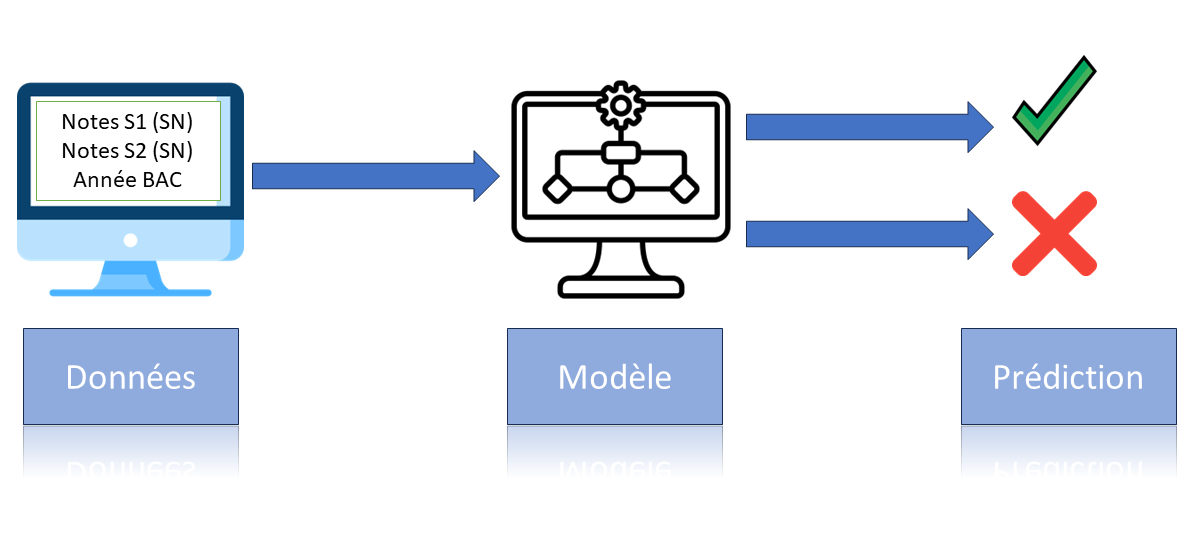
\includegraphics[width=10cm,height=6cm]{images/approce de solution.png}%
    }
    \caption{Approche de solution.}%
\end{figure}

\subsection{Choix des données et des caractéristiques pertinentes}
Pour notre modèle de prédiction, nous avons sélectionné un ensemble de données comprenant les notes des étudiants dans les matières clés du programme de licence économie, les années du baccalauréat, ainsi que d'autres caractéristiques pertinentes. Nous pensons que ces caractéristiques peuvent jouer un rôle important dans la prédiction de la réussite des étudiants en licence économie, en nous permettant de capturer à la fois les aspects académiques et non académiques qui peuvent influencer les performances des étudiants.

\subsection{Résultats attendus}
Les résultats que nous espérons obtenir de notre modèle de prédiction de la réussite des étudiants en licence économie sont basés sur nos objectifs initiaux.

Nous nous attendons à ce que notre modèle soit capable de prédire avec une précision élevée la probabilité de réussite des étudiants en licence économie. Nous visons une précision minimale de 70\% sur notre ensemble de données de test, ce qui signifie que le modèle doit être capable de classer correctement au moins 70\% des étudiants dans la bonne catégorie (réussite ou échec).

Nous attendons également d'évaluer les performances de notre modèle en mettant l'accent sur sa capacité à prédire de manière précise la réussite des étudiants indépendamment du type de licence.

Enfin, nous attendons d'analyser les facteurs prédictifs de la réussite des étudiants en licence économie, en identifiant les caractéristiques les plus importantes pour prédire leur réussite. Cela nous permettra de mieux comprendre les déterminants du succès des étudiants et de fournir des recommandations pour améliorer les taux de réussite.

\section{Modélisation}

\subsection{Choix du modèle}
Le choix du modèle de prédiction repose sur plusieurs critères, notamment la nature des données disponibles, la complexité du problème et les performances attendues. Dans notre étude, nous avons opté pour un modèle d'apprentissage supervisé en raison de la disponibilité de données étiquetées sur les réussites des étudiants en licence économie. Plus précisément, nous avons choisi d'utiliser des algorithmes de classification, car notre objectif est de prédire la probabilité de réussite des étudiants en les classant dans différentes catégories (réussite ou échec).

\subsection{Analyse et méthodes de prétraitement des données}
Avant d'entamer le processus d'entraînement de notre modèle de prédiction, une analyse approfondie de nos données s'est imposée.
L'analyse de la forme de nos données révèle un ensemble de 5655 étudiants et 31 colonnes. Parmi ces colonnes, 25 sont de type réel, 4 sont de type entier, et 3 sont de type objet ou chaîne de caractères, comprenant des informations telles que le nom, le prénom et le matricule des étudiants. 

\begin{table}[H]%
    \center%
    \setlength{\fboxsep}{5pt}%
    \setlength{\fboxrule}{0.5pt}%
    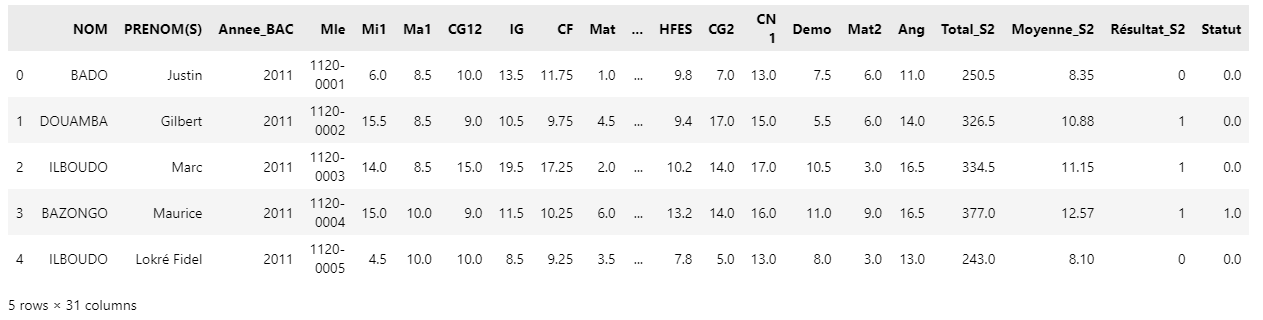
\includegraphics[width=11cm,height=3cm]{images/Dataset.png}%
    \caption{Présentation du Dataset.}%
\end{table}

Sur l’ensemble de ces données, nous avons un manque de données au niveau de la variable cible, soit environ 36\% des données sont manquantes. Ce manque est lié à l’indisponibilité des résultats de licence des bacheliers de 2017 et 2018.
Après avoir effectué une analyse approfondie de nos données, nous avons appliqué plusieurs méthodes de prétraitement des données pour garantir la qualité et la fiabilité de nos prédictions. Cela inclut le nettoyage des données pour éliminer les valeurs aberrantes et les données manquantes, la normalisation des données pour mettre toutes les caractéristiques sur la même échelle, la sélection des caractéristiques pour éliminer les variables redondantes ou peu informatives, et la conversion des données catégorielles en format numérique si nécessaire. Ensuite, les données sont divisées en ensembles d'entraînement et de test pour évaluer les performances du modèle. En appliquant ces méthodes de prétraitement, nous avons amélioré la qualité de nos données et optimisé les performances de notre modèle de prédiction.
\begin{figure}[H]
    \centering
    \setlength{\fboxsep}{5pt}
    \setlength{\fboxrule}{0.5pt}
    \begin{minipage}[t]{0.45\textwidth}
        \centering
        \fbox{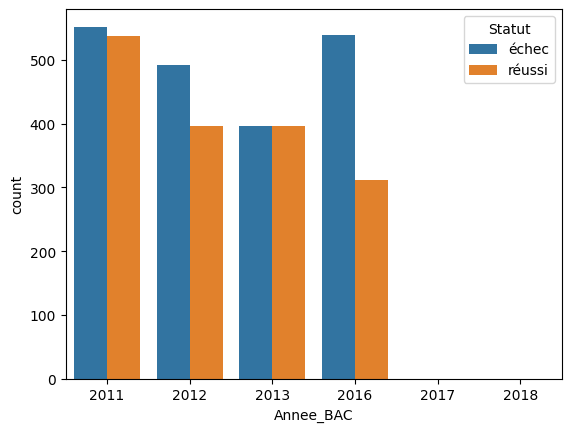
\includegraphics[width=7cm,height=5cm]{images/1.png}}
        \caption{Histogramme des valeurs manquantes pour les BAC 2017 et BAC 2018 avant le prétraitement.}
    \end{minipage}\hfill
    \begin{minipage}[t]{0.45\textwidth}
        \centering
        \fbox{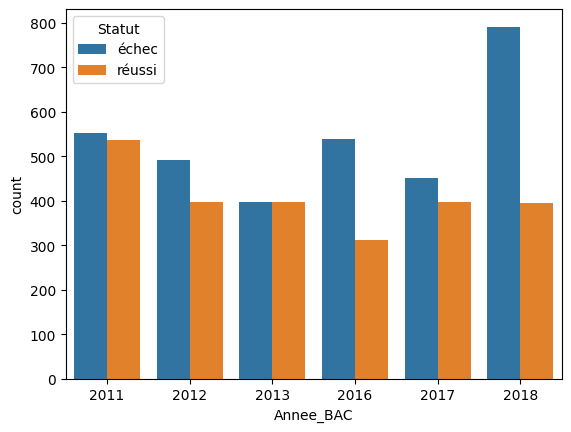
\includegraphics[width=7cm,height=5cm]{images/2.png}}
        \caption{Histogramme des valeurs manquantes pour les BAC 2017 et BAC 2018 après le prétraitement.}
    \end{minipage}
\end{figure}


\subsection{Entraînement du modèle}
L'étape d'entraînement du modèle implique de présenter les données d'entraînement à chacun des algorithmes sélectionnés et d'ajuster leurs paramètres en utilisant différentes techniques d'optimisation adaptées à chaque algorithme.
Les algorithmes entraînés sont entre autres:

\subsubsection{K plus proches voisins (KNN)}
L'algorithme des k plus proches voisins, également connu sous le nom de KNN ou k-NN, est un discriminant d'apprentissage supervisé non paramétrique, qui utilise la proximité pour effectuer des classifications ou des prédictions sur le regroupement d'un point de données individuel. Bien qu'il puisse être utilisé pour des problèmes de régression ou de classification, il est généralement utilisé comme algorithme de classification, en partant de l'hypothèse que des points similaires peuvent être trouvés les uns à côté des autres.
\begin{figure}[H]%
    \center%
    \setlength{\fboxsep}{5pt}%
    \setlength{\fboxrule}{0.5pt}%
    \fbox{
    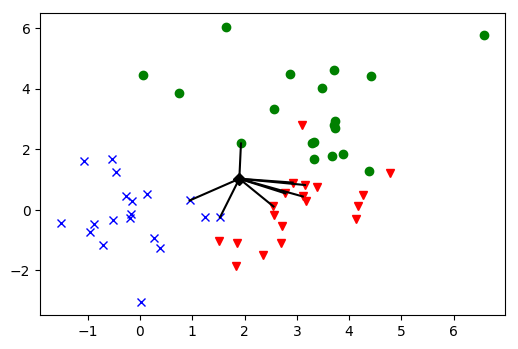
\includegraphics[width=11cm,height=6cm]{images/KNN.png}%
    }
    \caption{K plus proches voisins.}%
\end{figure}


\subsubsection{Machines à vecteurs de support (SVM)}
Les machines à vecteurs de support, de l'anglais Support Vector Machines, sont aussi appelées Séparateur à Vaste Marge. Ce sont des algorithmes d'apprentissage qui servent à prévoir une variable quantitative. Elles permettent de classer ou séparer les données en étant le plus éloigné possible des observations. En effet, il peut y avoir une infinité de séparateurs possibles. Le meilleur hyperplan est, selon les SVMs celui qui maximise les marges avec les objets de chaque catégorie.
\begin{figure}[H]%
    \center%
    \setlength{\fboxsep}{5pt}%
    \setlength{\fboxrule}{0.5pt}%
    \fbox{
    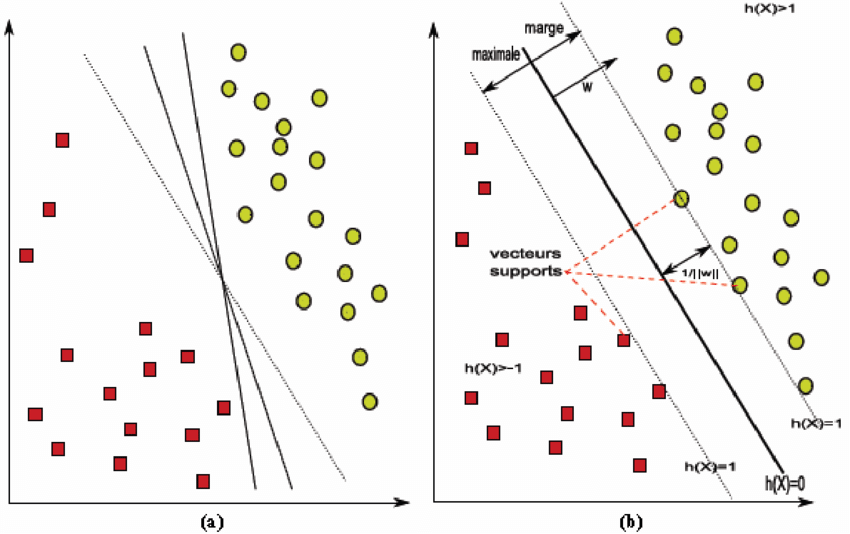
\includegraphics[width=12cm,height=7cm]{images/Principe-des-SVM.png}%
    }
    \caption{Machines à vecteurs de support.}%
\end{figure}

\subsubsection{Arbres de décision}
Les arbres de décision sont un modèle de prédiction qui peut être représenté sous la forme d’un arbre. Chaque nœud de l’arbre teste une condition sur une variable et chacun de ses enfants correspond à une réponse possible à cette condition. Les feuilles de l’arbre correspondent à une étiquette.
Pour prédire l’étiquette d’une observation, on « suit » les réponses aux tests depuis la racine de l’arbre, et on retourne l’étiquette de la feuille à laquelle on arrive.
\begin{figure}[H]%
    \center%
    \setlength{\fboxsep}{5pt}%
    \setlength{\fboxrule}{0.5pt}%
    \fbox{
    \includegraphics[width=12cm,height=5cm]{images/abre de décision.png}%
    }
    \caption{Exemple d’arbre de décision pour étiqueter un fruit.}%
\end{figure}

\subsubsection{Réseaux de neurones artificiels}
Les réseaux de neurones, également connus sous le nom de réseaux de neurones artificiels (ANN) ou réseaux de neurones simulés sont au cœur des algorithmes de l'apprentissage en profondeur. Leur nom et leur structure sont inspirés du cerveau humain, imitant la manière dont les neurones biologiques s'envoient des signaux.
Les réseaux de neurones artificiels sont constitués de couches nodales, contenant une couche d'entrée, une ou plusieurs couches cachées et une couche de sortie. Chaque nœud, ou neurone artificiel, se connecte à un autre et possède un poids et un seuil associés. Si la sortie d'un nœud est supérieure à la valeur de seuil spécifiée, ce nœud est activé et envoie des données à la couche suivante du réseau. Sinon, aucune donnée n'est transmise à la couche suivante du réseau.
\begin{figure}[H]%
    \center%
    \setlength{\fboxsep}{5pt}%
    \setlength{\fboxrule}{0.5pt}%
    \fbox{
    \includegraphics[width=10cm,height=6cm]{images/Réseaux de neurones.png}%
    }
    \caption{Réseaux de neurones artificiels.}%
\end{figure}

\subsubsection{Adaboost}
L'algorithme AdaBoost, ou Adaptive Boosting, est une technique d'apprentissage automatique utilisée principalement pour la classification. Son principe de fonctionnement repose sur l'idée de combiner plusieurs classificateurs faibles pour former un classificateur fort. Initialement, chaque exemple de formation se voit attribuer un poids égal. Ensuite, AdaBoost itère sur les données d'entraînement, en accordant une attention particulière aux exemples mal classés par les classificateurs précédents. À chaque itération, un nouveau classificateur faible est entraîné, et les poids des exemples sont mis à jour en fonction de leurs erreurs de classification. Les classificateurs faibles sont ensuite pondérés en fonction de leur performance, et leur combinaison conduit à un classificateur global.
\begin{figure}[H]%
    \center%
    \setlength{\fboxsep}{5pt}%
    \setlength{\fboxrule}{0.5pt}%
    \fbox{
    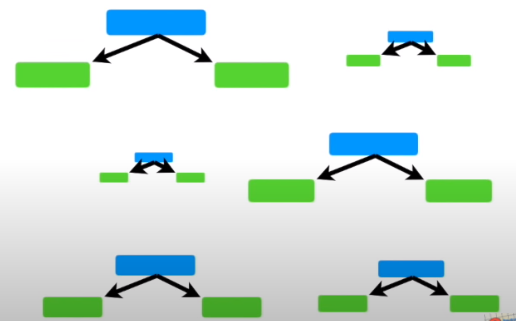
\includegraphics[width=10cm,height=6cm]{images/Adaboost img.png}%
    }
    \caption{Adaboost.}%
\end{figure}

\subsubsection{Forêt aléatoire}
La forêt aléatoire est un algorithme d'apprentissage automatique utilisé pour la classification, la régression et d'autres tâches. Elle appartient à la famille des méthodes d'ensemble, tout comme AdaBoost. La forêt aléatoire crée un ensemble de nombreux arbres de décision, où chaque arbre est formé sur un sous-ensemble aléatoire des données d'entraînement et utilise une sélection aléatoire des caractéristiques à chaque nœud de décision. L'idée principale derrière la forêt aléatoire est que la combinaison des prédictions de plusieurs arbres de décision réduit le surapprentissage et améliore la performance prédictive du modèle global.
\begin{figure}[H]%
    \center%
    \setlength{\fboxsep}{5pt}%
    \setlength{\fboxrule}{0.5pt}%
    \fbox{
    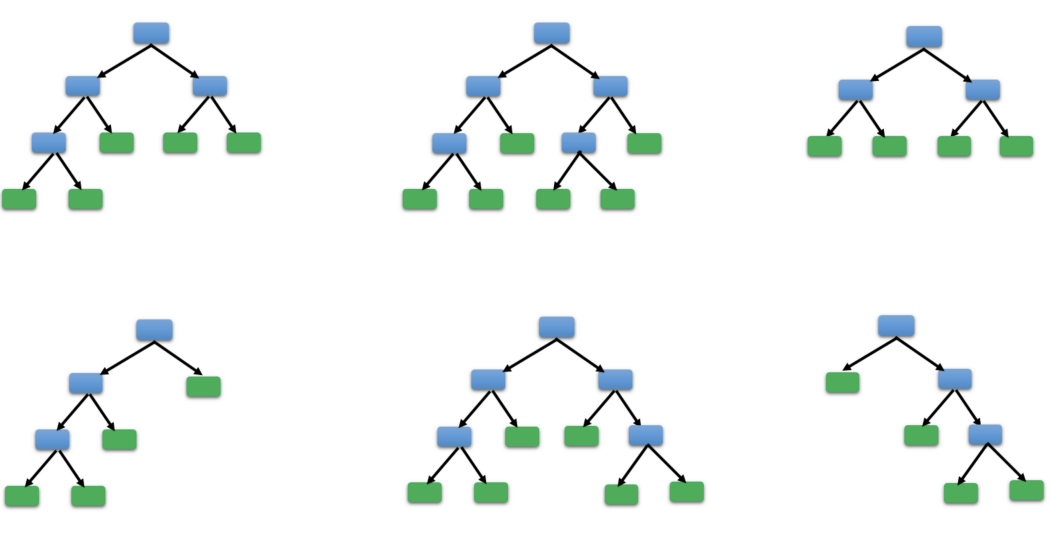
\includegraphics[width=10cm,height=6cm]{images/rand_forest_illustration.png}%
    }
    \caption{Forêt aléatoire.}%
\end{figure}

Chaque algorithme apprend à partir des exemples d'entraînement en ajustant ses paramètres internes de manière à minimiser la fonction de perte spécifique à chaque algorithme, ce qui lui permet de généraliser et de faire des prédictions précises sur de nouvelles données.

\section{Conclusion}
Ce chapitre nous a permis d'explorer l'état de l'art sur la prédiction de la réussite des étudiants, en examinant les études antérieures, les méthodes et techniques utilisées, ainsi que les limitations des approches existantes. Nous avons également présenté une approche de solution visant à prédire le succès universitaire des étudiants orientés en économie, en utilisant l'intelligence artificielle, et la modélisation de cette solution, notamment le choix du modèle, la méthode de prétraitement des données et l'entraînement du modèle, offrant ainsi un aperçu de la méthodologie à suivre pour mener à bien cette prédiction.
